% !TEX TS-program = pdflatex
% !TEX encoding = UTF-8 Unicode

% TeX-M (r1.1)
% For my math classes at UT Austin
% Notes template created by Abdon Morales for the College of Natural Science
% and for the Department of Mathematics and Computer Science
% (c) 2019 - 2024 Abdon Morales and the University of Texas at Austin
% This is a notes template for a LaTeX document using the "article" class for Mathematics (Calculus)
% at the University of Texas at Austin.

% Last change made: Jan 27, 2024 1:40 AM CST

% See "book", "report", "letter" for other types of document.

\documentclass[11pt]{article} % use larger type; default would be 10pt

% Start of Article customization options and addons (for more help and information reference to Overleaf's guides and docs on Latex.
\usepackage[utf8]{inputenc} % set input encoding (not needed with XeLaTeX)

%%% Examples of Article customizations
% These packages are optional, depending whether you want the features they provide.
% See the LaTeX Companion or other references for full information.

%%% PAGE DIMENSIONS
\usepackage{geometry} % to change the page dimensions
\geometry{letterpaper} % or letterpaper (US) or a5paper or....
% \geometry{margin=2in} % for example, change the margins to 2 inches all round
% \geometry{landscape} % set up the page for landscape
%   read geometry.pdf for detailed page layout information

\usepackage{graphicx} % support the \includegraphics command and options
\usepackage{xcolor}

% \usepackage[parfill]{parskip} % Activate to begin paragraphs with an empty line rather than an indent

%%% PACKAGES
\usepackage{booktabs} % for much better looking tables
\usepackage{array} % for better arrays (eg matrices) in maths
\usepackage{paralist} % very flexible & customisable lists (eg. enumerate/itemize, etc.)
\usepackage{verbatim} % adds environment for commenting out blocks of text & for better verbatim
\usepackage{subfig} % make it possible to include more than one captioned figure/table in a single float
\usepackage{exercise}
% Math tools
\usepackage{mathtools}
\usepackage{amsmath}
\usepackage{tikz} % For charts, mathematical graphs, and etc
%% Equal symbol for L'Hospital Rule
\usepackage{tcolorbox}
\newcommand\LR{\stackrel{\mathclap{\normalfont\mbox{L.R}}}{=}}
% These packages are all incorporated in the memoir class to one degree or another...

%%% HEADERS & FOOTERS
\usepackage{fancyhdr} % This should be set AFTER setting up the page geometry
\pagestyle{fancy} % options: empty , plain , fancy
\renewcommand{\headrulewidth}{0pt} % customise the layout...
\lhead{}\chead{}\rhead{}
\lfoot{}\cfoot{\thepage}\rfoot{}

%%% SECTION TITLE APPEARANCE
\usepackage{sectsty}
\allsectionsfont{\sffamily\mdseries\upshape} % (See the fntguide.pdf for font help)
% (This matches ConTeXt defaults)

%%% ToC (table of contents) APPEARANCE
\usepackage[nottoc,notlof,notlot]{tocbibind} % Put the bibliography in the ToC
\usepackage[titles,subfigure]{tocloft} % Alter the style of the Table of Contents
\renewcommand{\cftsecfont}{\rmfamily\mdseries\upshape}
\renewcommand{\cftsecpagefont}{\rmfamily\mdseries\upshape} % No bold!
%%% Question creation
\renewcommand\ExerciseName{Question~}
\renewcommand\AnswerName{Answer to question}
\renewcommand\ExerciseHeader{%
  \noindent\parbox[t]{.18\textwidth}{%
    \bfseries\large\ExerciseName\ExerciseHeaderNB\hfill}%
  \parbox[t]{.72\textwidth}{%
    \centering\bfseries\large%
    \ExerciseHeaderTitle\ExerciseHeaderOrigin}%
  \par\medskip
}
%%% END Article customizations

%%% The "real" document content comes below...

% Replace examples with the actual content you intend to put
\title{International Trade}
\author{Abdon Morales \\ The University of Texas at Austin \\ ECO 304L \\ Wayne Geerling}
\date{\today \\ Chapter 19 : Week 13}
%\date{} % Activate to display a given date or no date (if empty),
         % otherwise the current date is printed 

\begin{document}
\maketitle
\section*{\textbf{Nations gain through international trade, even if they can produce their goods and services domestically.}}
It's often assumed that, if possible, nations should try to produce their own goods and services rather than trade for them. For many, it seems intuitive that if the United States \textit{can} produce a particular good, the United States \textit{should} produce that good; but way back in Chapter 2, we learned that how individuals gain by specializing in the production of certain goods and obtaining other goods through trade, even when the individuals could produce those other goods more efficiently themselves. Here we will see how the same principles apply to trade between nations. This second look at trade will give us a chance to go deeper into the theory.

International trade is greatly facilitated by an invention that gets little fanfare: the stackable shipping container, conceived and developed in the mid-1950s by trucking magnate Malcolm McLean and engineer Keith Tantlinger. Prior to that time, ships had cargo holds; wooden crates of cargo were loaded individually and meticulously fitted together like a jigsaw puzzle, to maximize the use of interior space. All of this took time, and more time on the unloading end; McLean and Tantlinger's inspired insight was that on- and off-loading time could be reduced dramatically by using metal containers of uniform size and shape, and using large cranes to stack the containers, securely locked together, on the decks of specially configured ships, instead down in the holds.

Today every container is geo-tagged, so manufacturing plants know exactly when the components they need are off-loaded. This arrangement makes just-in-time manufacturing possible; overall, the "containerization" of shipping reduced costs by approximately 35\% compared to the use of cargo holds. The past few decades have seen the volume of trade among the world's nations rise dramatically, though bottlenecks caused by coronavirus-related impacts have shown weaknesses in this model.

To help illustrate the extent of international trade, we begin this chapter with a look at global trade data. We then consider how international trade affects an economy; finally, we have to reckon with the fact that, despite the theoretical arguments for free trade and the practical advances that makes it easy and cheap, not everyone is convinced that free trade is a good. So we conclude the chapter by examining trade barriers and the reasons for their existence.

\begin{tcolorbox}[width=\textwidth,colback={white},title={Big Questions},colbacktitle=yellow,coltitle=blue]
\begin{itemize}
\item Is globalization for real?
\begin{itemize}
\item Over the long run, yes, globalization is very real. Since 1970, world exports have grown from 10\% to about 22\% of world GDP; for the United States, imports and exports have both grown over the past five decades. However, this trend has slowed and maybe even reversed since about 2010; the Great Recession slowed world trade, and then Trump-era trade restrictions imposed by both the United States and foreign governments slowed it further.
\end{itemize}
\item How does international trade help the economy?
\begin{itemize}
\item Gains from trade occur when a nation specializes in production and exchanges its output with a trading partner. For this arrangement to work, each nation must produce goods for which it is a low-opportunity-cost producer and then trade them for goods for which it is a high-opportunity-cost producer.
\item In addition, trade benefits nations' economies through economies of scale and increased international competition 
\end{itemize}
\item What are the effects of tariffs and quotas?
\begin{itemize}
\item Protectionism in the form of trade restrictions, such as tariffs and quotas, is common; a tariff is a tax on imports. A quota is a quantity restriction on imports.
\item Proponents of trade restrictions often cite the need to protect defense-related industries and fledgling firms and to fend off dumping; but protectionist policies can also serve as political favors to special interest groups.
\end{itemize}
\end{itemize}
\end{tcolorbox}

\section*{\textbf{Is globalization for real?}}
Imports and exports are both up for other countries, as well, and that means economies around the globe are more and more interdependent. This interdependence is the essence of \textit{globalization}, and it is changing not only what you purchase but also your future job prospects.

The modern trade explosion has occurred for many reasons; among these are lower shipping and communication costs, reduced trade barriers, and increased specialization in world economies. Total world exports of goods and services are now about one-fourth the size of world GDP. In this section, we look first at the growth in total world trade and then at trends in U.S trade.

\subsection*{Growth in World Trade}
World trade has grown, but not just in market value; it has also grown as a percentage of total world output. That is, not only are nations trading more, but they are also trading a greater portion of their GDP. Figure 19.1 shows merchandise trade as a percentage of world GDP; this has expanded dramatically, nearly doubling over 50 years, from 11\% in 1970 to 21\% in 2020.

\begin{center}
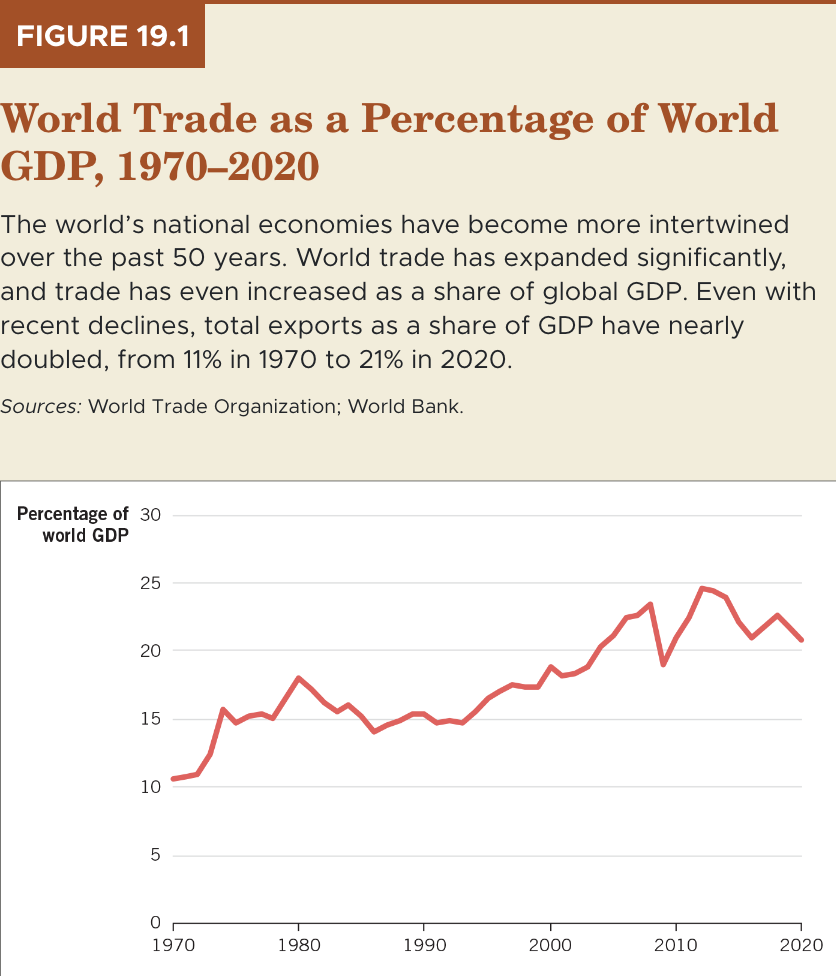
\includegraphics[scale=0.5]{images/Figure 19.1.png} 
\end{center}
\subsection*{Trends in U.S trade}
Trends in U.S international trade are similar to overall global trends; the United States is the world's biggest economy. A huge amount of trade takes place between the individual states \textit{inside} the country. Still, even with the ability to produce and trade so much within U.S borders, the nation's participation in international trade has risen dramatically in recent years. Figure 19.2 shows U.S exports and imports as a percentage of GDP from 1970 to 2020.

\begin{center}
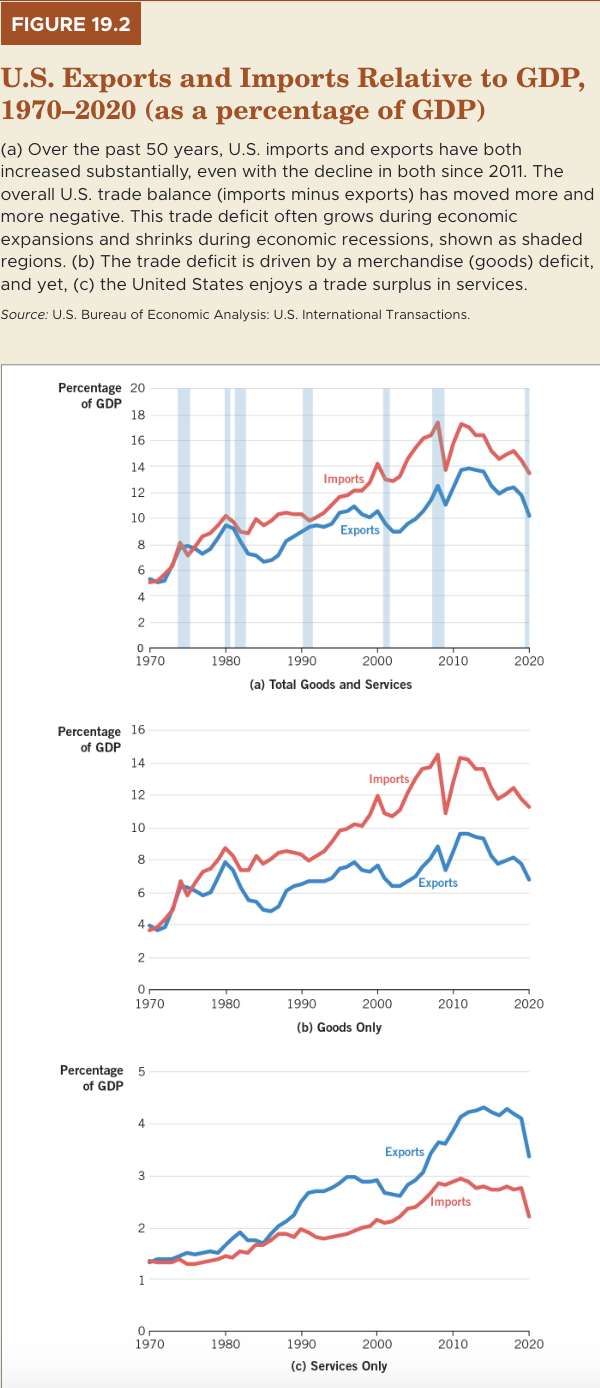
\includegraphics[scale=0.5]{images/Figure 19.2.png} 
\end{center}
As you look at the data in Figure 19.2, note three features; first, in panel (a), notice that both imports and exports increased significantly over the 50 years from 1970 to 2020. However, this trend toward globalization has leveled off in the past few years; part of this is the effects of the Great Depression from 2007 to 2009. Another important factor is the increase in trade barriers that began during the Trump administration and have not yet been eliminated. Since 2011, U.S imports and exports have both fallen relative to GDP; further, shipping disruptions caused by the coronavirus pandemic have caused some to wonder if the length of supply chains will decrease and become more local.

Second, since 1975, U.S imports have exceeded U.S exports; \textbf{\textcolor{red}{net exports}} is the total exports of final goods and services minus total imports of final goods and services. The difference between a nation's total exports and total imports is its \textbf{\textcolor{red}{trade balance}}. If a nation exports more than it imports, it has a positive trade balance, or a \textbf{\textcolor{red}{trade surplus}}. However, if a nation imports more than it exports, it has a negative trade balance, or a \textbf{\textcolor{red}{trade deficit}}.

Panel (c) of Figure 19.2 reveals a little-known fact about U.S trade: while the merchandise (good) trade deficit is very large, the United States actually has a service trade surplus. Popular U.S service exports include financial, travel, and education services. 

Finally, notice how the business cycle affects international trade; during recessionary periods (indicated by the light blue bars in Figure 19.2a), imports generally drop. As the economy recovers, imports begin to rise again; in addition, while exports often drop during recessions, the trade deficit tends to shrink during downturns. Part of this fluctuation reflects the way imports and exports are calculated; in short, note the strong relationship between trade and economic activity: trade generally expands during economic expansions and contracts during recessions.

\subsection*{Major trading partners of the United States}
Figure 19.3 shows the value of imports from and exports to these top nine trading partners of the United States.

In the past, our closest neighbors - Canada and Mexico - were our chief trading partners. From Canada we get motor vehicles, oil, natural gas, and many other goods and services; from Mexico we get motor vehicles, coffee, computers, household appliances, and gold. More recently, falling transportation costs have led to increased trade from other countries, as well.

\begin{center}
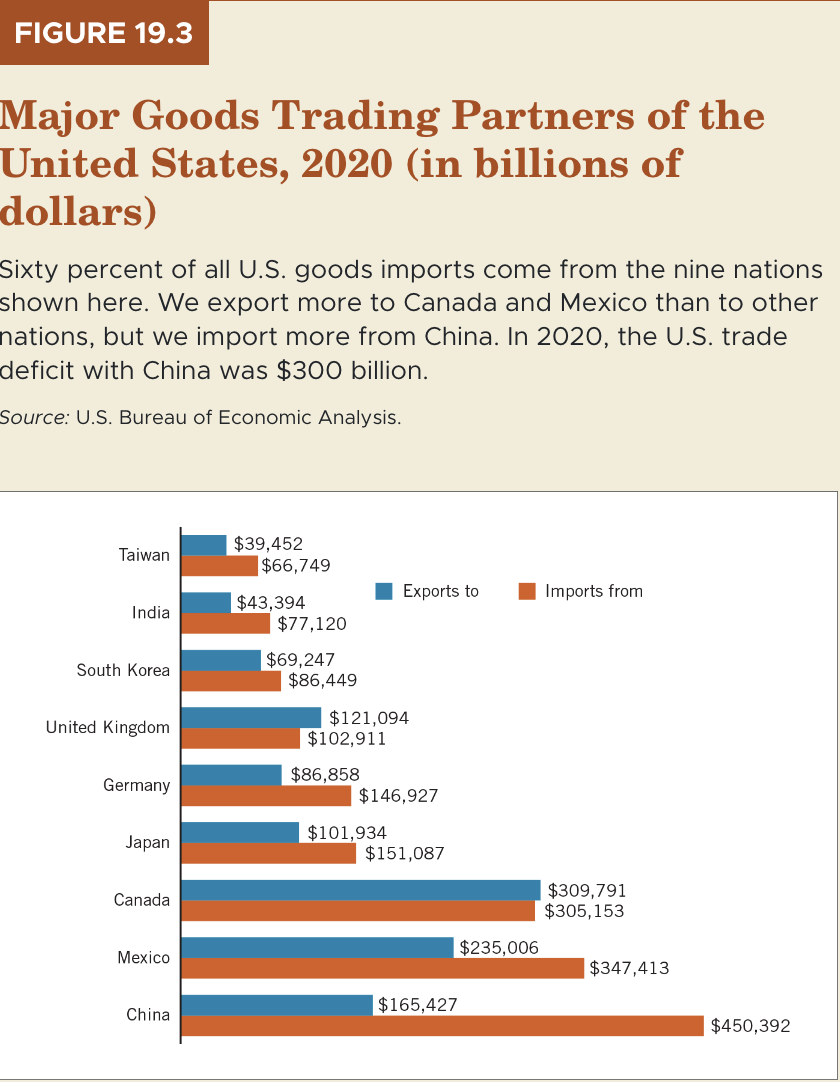
\includegraphics[scale=0.5]{images/Figure 19.3.png} 
\end{center}
Canada and Mexico buy the most exports; to Canada we export cars, car parts, computers, and agricultural products. To Mexico we export cars, car parts, computers, and meat, among many other items; financial and travel services are major U.S exports to all our major trading partners.

\section*{\textbf{How does international trade help the economy?}}
In this section, we explain how comparative advantage and specialization make it possible to achieve gains from trade between nations.

\subsection*{Comparative Advantage}
In Chapter 2, we saw that trade creates value and that \textbf{\textcolor{red}{comparative advantage}} makes the creation of value possible. Gains arise when a nation specializes in production and exchanges its output with a trading partner; in other words, each nation should produce the good it is best at making and trade with other nations for the goods they are best at making. Trade leads to lower costs of production and maximizes the combined output of all nations involved. (Comparative advantage is very important to the discussion that follow. If you don't remember the details of comparative advantage, be sure to review Chapter 2 before proceeding

\begin{center}
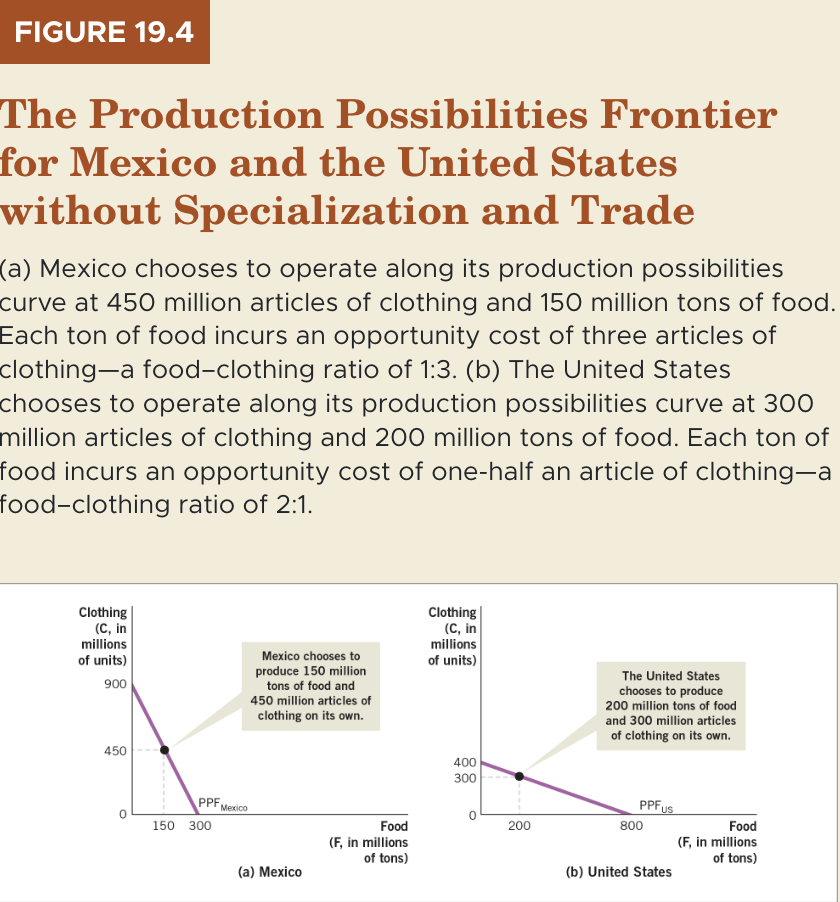
\includegraphics[scale=0.5]{images/Figure 19.4.png} \\
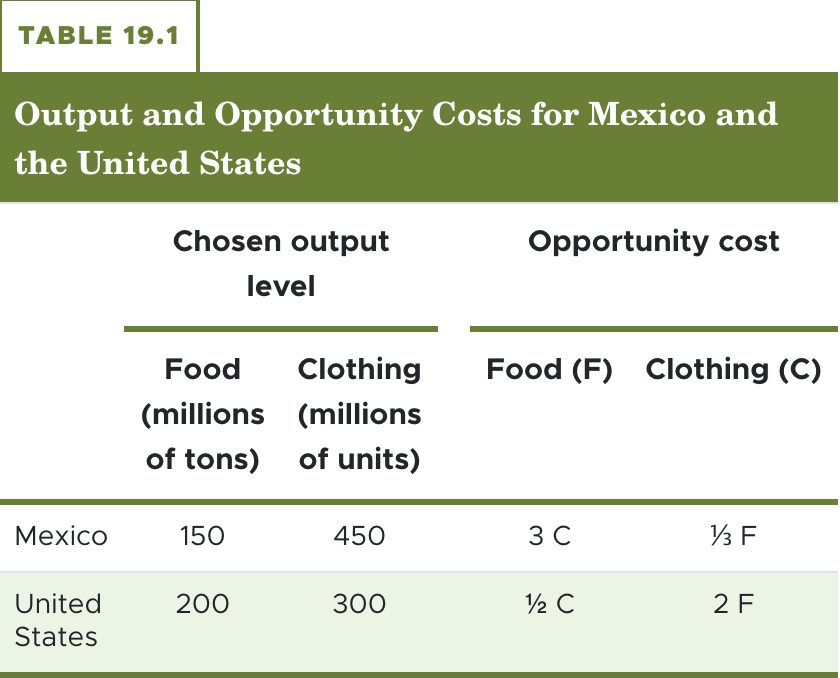
\includegraphics[scale=0.5]{images/Table 19.1.png} \\
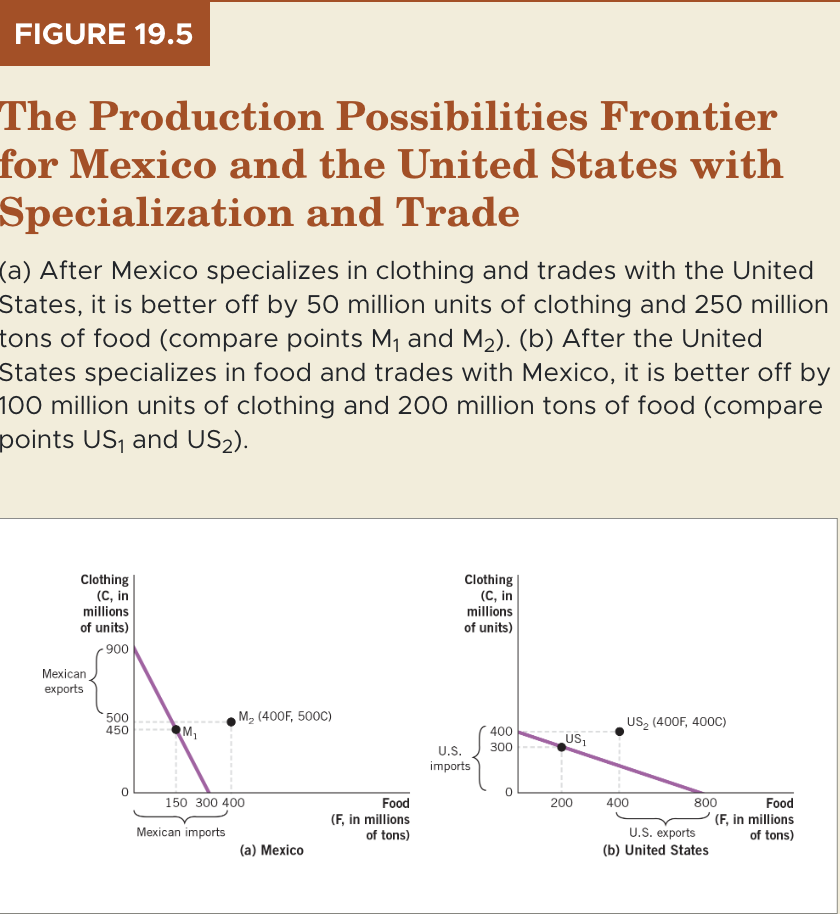
\includegraphics[scale=0.5]{images/Figure 19.5.png} 
\end{center}

The combined benefits that Mexico and the United States enjoy are even more significant; as we saw in Figure 19.4, when Mexico did not specialize and trade, it chose to make 450 million units of clothing and 150 million tons of food. Without specialization and trade, the United States chose to produce 300 million units of clothing and 200 million tons of food. The combined output without specialization was 750 million units of clothing and 350 million tons of food. However, as we see in Figure 19.5, the joint output with specialization is 900 million units of clothing and 800 millions tons of food; in economics, we call this a \textit{positive-sum game} because both players, in this case both countries, win by trading with each other.

\subsection*{Other Advantages of Trade}
Although comparative advantage is the biggest reason that many nations trade with other nations, there are other good reasons for nations to engage trade. In this section, we consider how international trade encourages both economies of scale and increase competition and how these factors can help an economy to grown.
\subsubsection*{\textcolor{olive}{Economies of Scale}}
\subparagraph*{
When a nation specializes its production, it can take advantage of the lower production costs that can accompany large-scale production processes. Economies of scale are especially important for smaller nations that do not have a population big enough to support the domestic production of large-scale items such as automobiles, television sets, steel, and aluminum. However, once a smaller nation has free access to larger markets, it can effectively specialize in what it does best and generate low per-unit costs through exports.}
\subparagraph*{
In Figure 19.4 and 19.5, the production possibilities frontier is shown as a straight line, which makes the computation of the ratios fairly simple and holds the opportunity cost constant. However, in the real world, access to new markets allow countries to take advantage of economies of scale and therefore lower per-unit costs as production expands. Increased production gives companies the opportunity to economize on distribution costs and marketing and to utilize assembly lines and other forms of automation.}
\subsubsection*{\textcolor{olive}{Trade Agreements}}
\subparagraph*{Gains from trade often spur nations to sign trade agreements, to reduce tariffs and clear the way for mutually beneficial exchange.}
\subparagraph*{Even though trade agreements often stipulate protections for particular industries (most notably, agriculture), they still increase trade between nations.}
\subparagraph*{The World Trade Organization (WTO) is an international organization that facilitates trade agreements between nations. Created in 1995 by 123 countries that were then signatories of the General Agreement on Tariffs and Trade, the WTO regulates the trade of various goods and services, including textiles, investment, intellectual property, even agriculture. Moreover, the WTO works to resolve trade disputes.}

\section*{\textbf{What are the effects of tariffs and quotas?}}
Despite the benefits of free trade, significant trade barriers, such as import taxes, often exist.
Import taxes like those on footwear are not unusual. In this section, we explore two of the most common types of trade barriers: \textit{tariffs} and \textit{quotas}; We then look more closely at common economic and political justification for \textbf{protectionism}, which is a blanket term for governmental actions and policies that restricts or restrain international trade, often with the intent of protecting local businesses and jobs from foreign competition. We close by examining whether or not protectionism is effective.
\subsection*{Tariffs}
\textbf{Tariffs} are taxed levied on imported goods and services; a tariff is paid by the producer of the good when the good arrives in a foreign country. A tariff can be a percentage of the value of the good (called an \textit{ad valorem tax}), a per-unit tax (called a \textit{specified tax}), or a mixed of the two. Figure 19.6 illustrate the impact of a per-unit tariff on foreign shoes; to assess how a tariff affects the market price of shoes in the United States, we observe the relationship between domestic demand and supply.

% Put image for Figure 19.6

\subsection*{Quotas}
Sometimes, instead of taxing imports, governments use import quotas to restrict trade. \textbf{Import quotas} are limits on the quantity of product that can be imported into a country; quotas function like tariffs with one crucial exception: the government does not receive any tax revenue. In the United States today, there are quotas on many products, including milk, tuna, olives, peanuts, cotton, and sugar.

%Add Figure 19.8

\subsection*{Reasons given for trade barriers}
Considering all that we have discussed about the gains form trade and the inefficiencies associated with tariffs and quotas, you might be surprised to learn that trade restrictions are quite common. In this section, we consider some of the reasons for the persistence of trade barriers; these include national security, protection of infant industries, retaliation for \textit{dumping}, and favors to special interests.
\subsubsection*{\textcolor{olive}{National Security}}
\subparagraph*{Many people believe that certain industries, such as weapons, energy, and transportation, are vital to our nation's defense. They argue that without the ability to produce its own missiles, firearms, aircraft, and other strategically significant assets, a nation could find itself relying on its enemies. Thus, people often argue that certain industries should be protected in the interest of national security.}
\subparagraph*{Although it is certainly important for any trade arrangement to consider national security, this argument has been used to justify trade restrictions on goods and services from nations with whom we have active, open trade relations.}
\subsubsection*{\textcolor{olive}{Infant Industries}}
\subparagraph*{Another argument in support of steel tariffs in the United States was that the U.S steel industry needed some time to implement new technologies that would enable it to compete with steel producers in other nations. This \textbf{infant industry argument} states that domestic industries need trade protection until they are established and able to compete internationally. According to this point of view, once the fledgling industry gains traction and can support itself, the trade restrictions can be removed. \\However, reality doesn't work this way; firms that lobby for protection are often operating in an established industry.}
\subsubsection*{\textcolor{olive}{Retaliation for dumping}}
\subparagraph*{\textbf{Dumping} occurs when a foreign supplier sells a good below the price it charges in its home country. As the name implies, dumping is often a deliberate effort to gain a foothold in a foreign market; it can also be the result of subsidies within foreign countries.}
\subparagraph*{In cases of dumping, the WTO allows for special \textit{countervailing duties} to offset the subsidies; thus, the United States placed a tariff on the imported tires to restore a level playing field. In essence, anytime a foreign entity decides to charge a lower price to penetrate a market, the country that is dumped on is likely to respond by imposing a tariff or quota to protect its domestic industries from foreign takeover. However, retaliation is also problematic; British economist Joan Robinson understood the risks well. She argued that the threat of trade barriers might conceivably work as a negotiation ploy, but when it came to actually enacting a retaliatory tariff, it "would be just as sensible to drop rocks into our harbours because other nations have rocky coasts."}
\subsubsection*{\textcolor{olive}{Favors to special interests}}
\subparagraph*{The imposition of trade barriers is often referred to as "protection"; this term raise the question...\textit{Who is being protected?} and \textit{What are they being protected from?} We have seen that trade barriers drive up domestic prices and lead to lower quantity of goods or services in the market where the barriers are imposed. This situation does not protect consumers; in fact, tariffs and quotas protect domestic producers from international competition. Steel tariffs were put in place to help domestic steel producers, and tire tariffs were put in place to help domestic tire producers.}
\subparagraph*{When we see trade barriers, the publicly stated reason is generally one of the three reasons we have already discussed: national security, infant industry protection, or retaliation for dumping; but we must also recognize that these barriers may be put in place as a favor to special interest groups that have much to gain at the expense of domestic consumers.}
\section*{Conclusion}
We began this chapter by rejecting the misconception that nations should not trade for goods and services they can produce for themselves. An analysis of the concept of comparative advantage shows that nations can gain by (1) specializing in the production of goods and services for which they have the lowest opportunity cost and then (2) trading for the other goods and services they wish to consume.

International trade expanding all over the world; the United States now imports and exports more than at any time in its history. Increased trade is generally positive for all nations involved; however, trade barriers still exist around the globe for various reasons, including national security, the protection of infant industries, retaliation for dumping and subsidies, and favors to special interests.
\end{document}